\documentclass[report.tex]{subfiles}

\externaldocument{report}

\begin{document}

\section{性能評価}

今回製作できたラジオは,以下のような仕様となった。

\begin{enumerate}
	\item ゲルマニウムダイオードを用いた検波を行うことができた。
	\item 4段のアンプを用いてスピーカーを駆動することができた。
	\item 多少の雑音はあるが、何を話しているのかを聞き取ることができた。
	\item ニッポン放送とTBSラジオと文化放送を受信することが出来たが複数の放送局が同時に聞こえる感じになってしまった。
	\item 可変抵抗を用いて音量調整を行うことができた。
	\item 直径24cm、高さ38cmのループアンテナを用いた一号機は持ち運びが困難であった。
	      しかし、直径6.5cm、高さ16.5cmのループアンテナを用いた二号機は少し受信感度が悪いが、持ち運びが容易であった。
	\item 教室(CAD室)内のどこでも受信できたが、ニッポン放送は窓側でないと聞き取れなかった。
\end{enumerate}

\subsection{検波}



\begin{figure}[H]
	\centering
	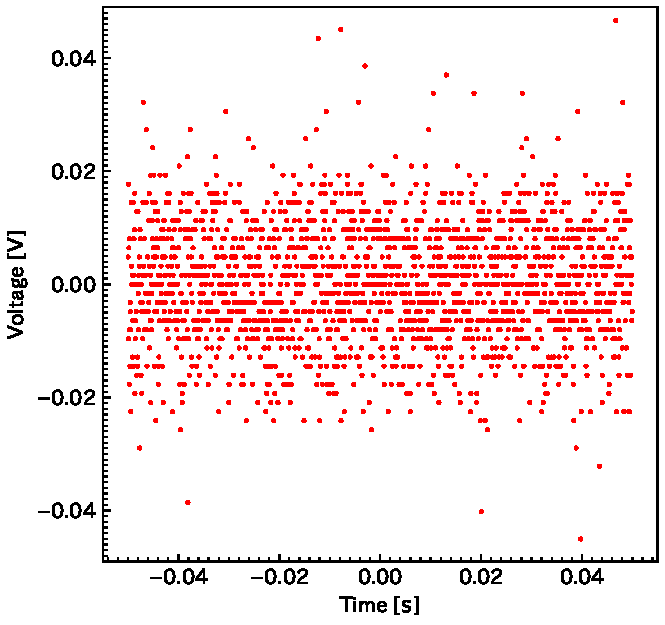
\includegraphics[width=7cm]{fig/koil.pdf}
	\caption{1号機アンテナの写真}
	\label{fig:koil}
\end{figure}

\begin{figure}[H]
	\begin{minipage}[b]{0.5\linewidth}
		\centering
		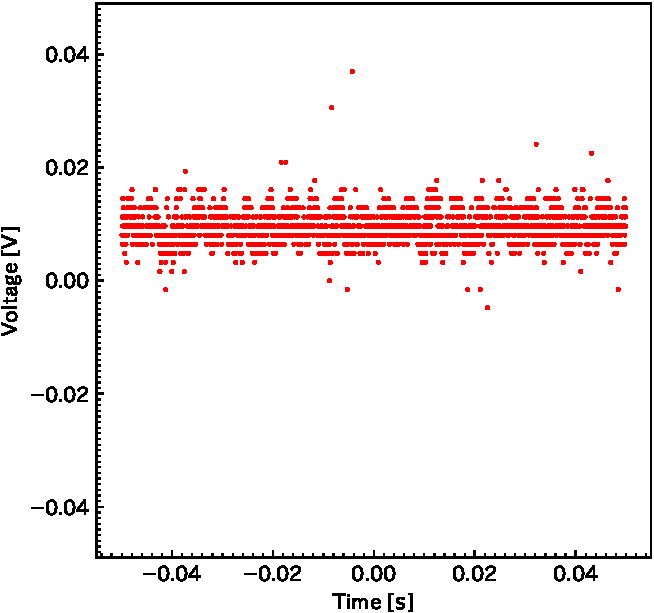
\includegraphics[width=7cm]{fig/koil_diode.pdf}
		\caption{2号機アンテナの写真}
		\label{fig:koil_diode}
	\end{minipage}
	\begin{minipage}[b]{0.5\linewidth}
		\centering
		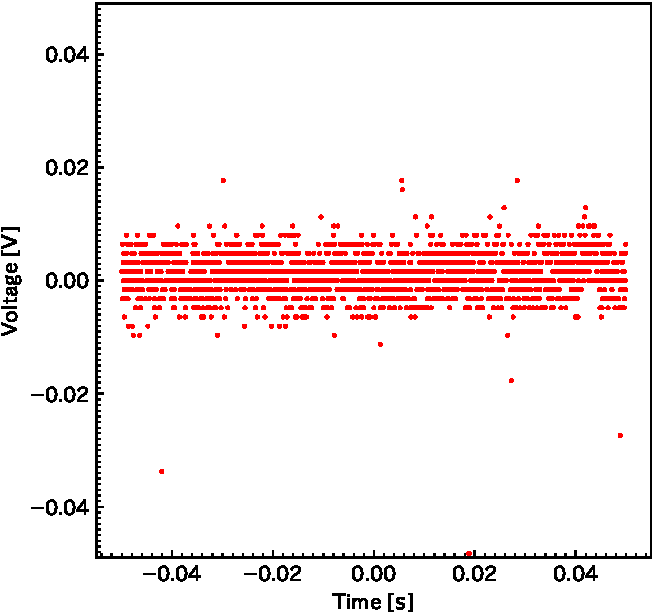
\includegraphics[width=7cm]{fig/koil_diode_bi.pdf}
		\caption{3号機アンテナの写真}
		\label{fig:koil_diode_bi}
	\end{minipage}
\end{figure}

\subsection{アンテナ}

今回は合計で3つのアンテナを用意した(1号機と2号機は製作したもの、3号機は既製品)。
それぞれの仕様を\wtab{ant}に示す。
また、それぞれの写真を\wfig{1},\wfig{2},\wfig{3}に示す。

\begin{table}[h]
	\centering
	\caption{アンテナの各パラメータ}
	\label{tab:ant}
	\begin{tabular}{ccccccc} \hline
		名称  & 直径[mm] & 巻き数[turn] & 抵抗[\(\Omega\)] & 長さ[mm] & コア材質  & コア長[mm] \\ \hline
		1号機 & 240    & 24        & 4.6            & 11     & 空気    & -       \\
		2号機 & 65     & 135       & 0.5            & 50     & 空気    & -       \\
		3号機 & 10     & 70        & 28.0           & 12     & フェライト & 42      \\ \hline
	\end{tabular}
\end{table}

\begin{figure}[H]
	\centering
	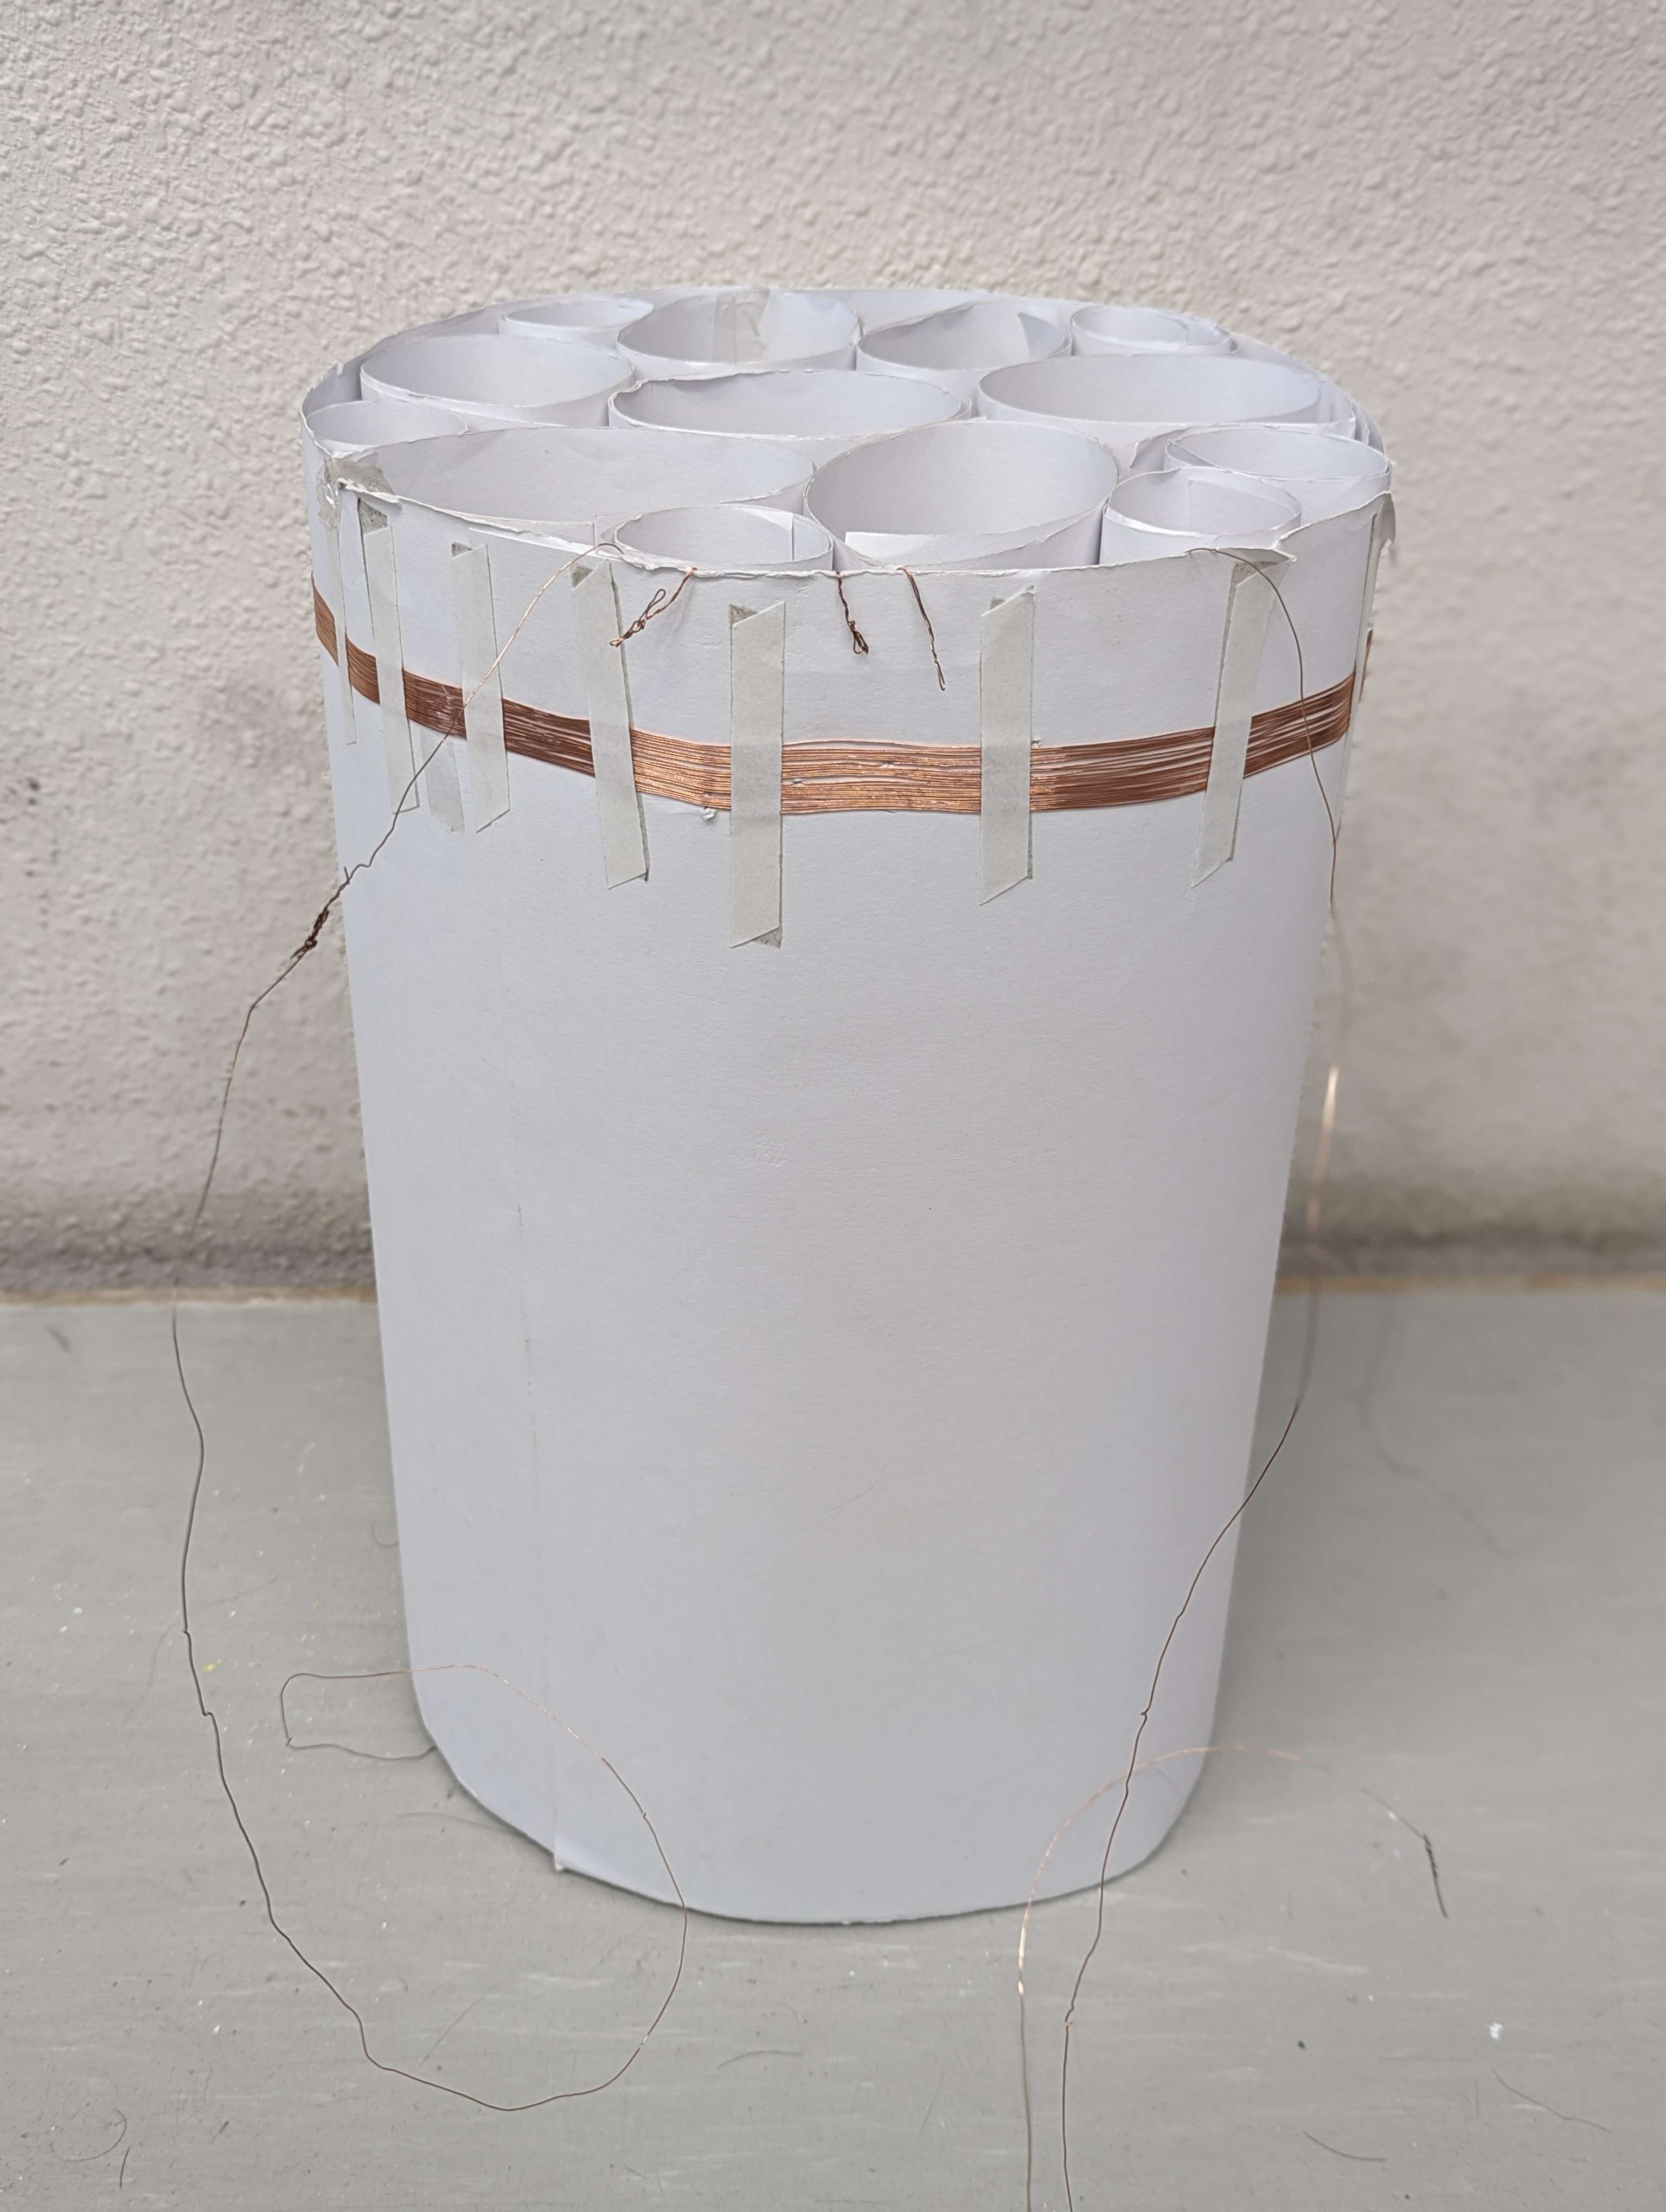
\includegraphics[width=7cm]{fig/1.jpg}
	\caption{1号機アンテナの写真}
	\label{fig:1}
\end{figure}

\begin{figure}[H]
	\begin{minipage}[b]{0.5\linewidth}
		\centering
		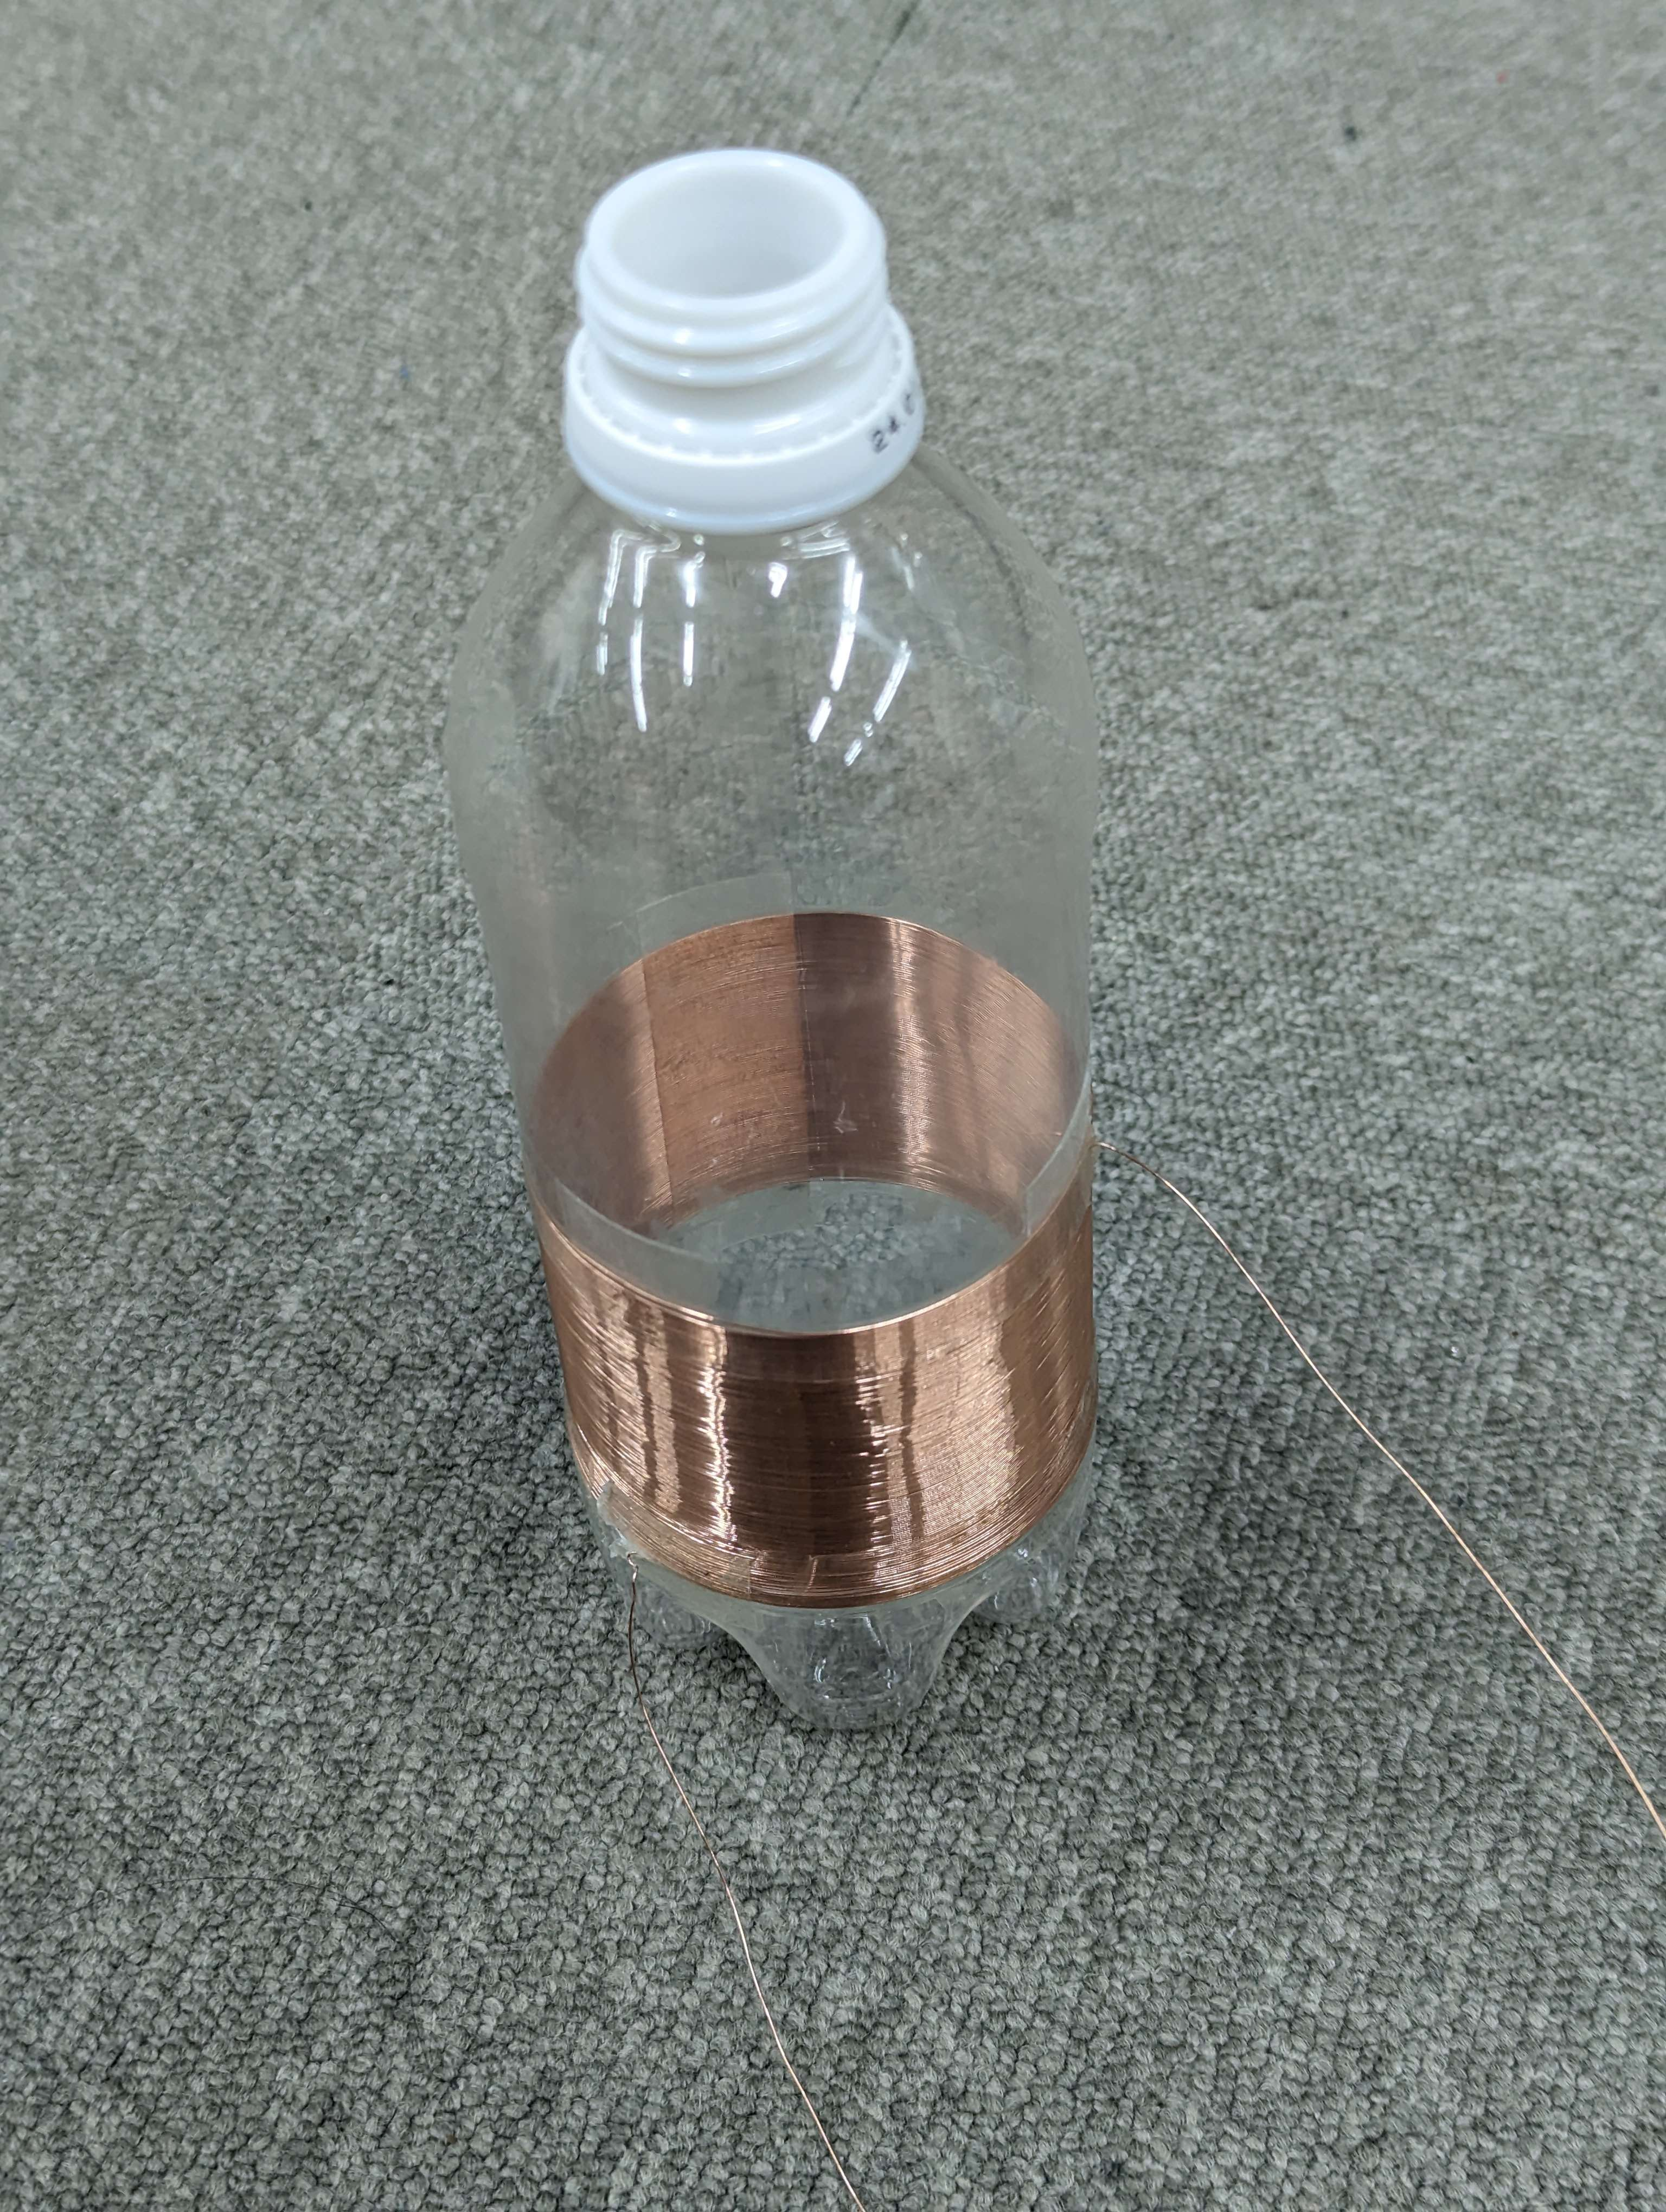
\includegraphics[width=7cm]{fig/2.jpg}
		\caption{2号機アンテナの写真}
		\label{fig:2}
	\end{minipage}
	\begin{minipage}[b]{0.5\linewidth}
		\centering
		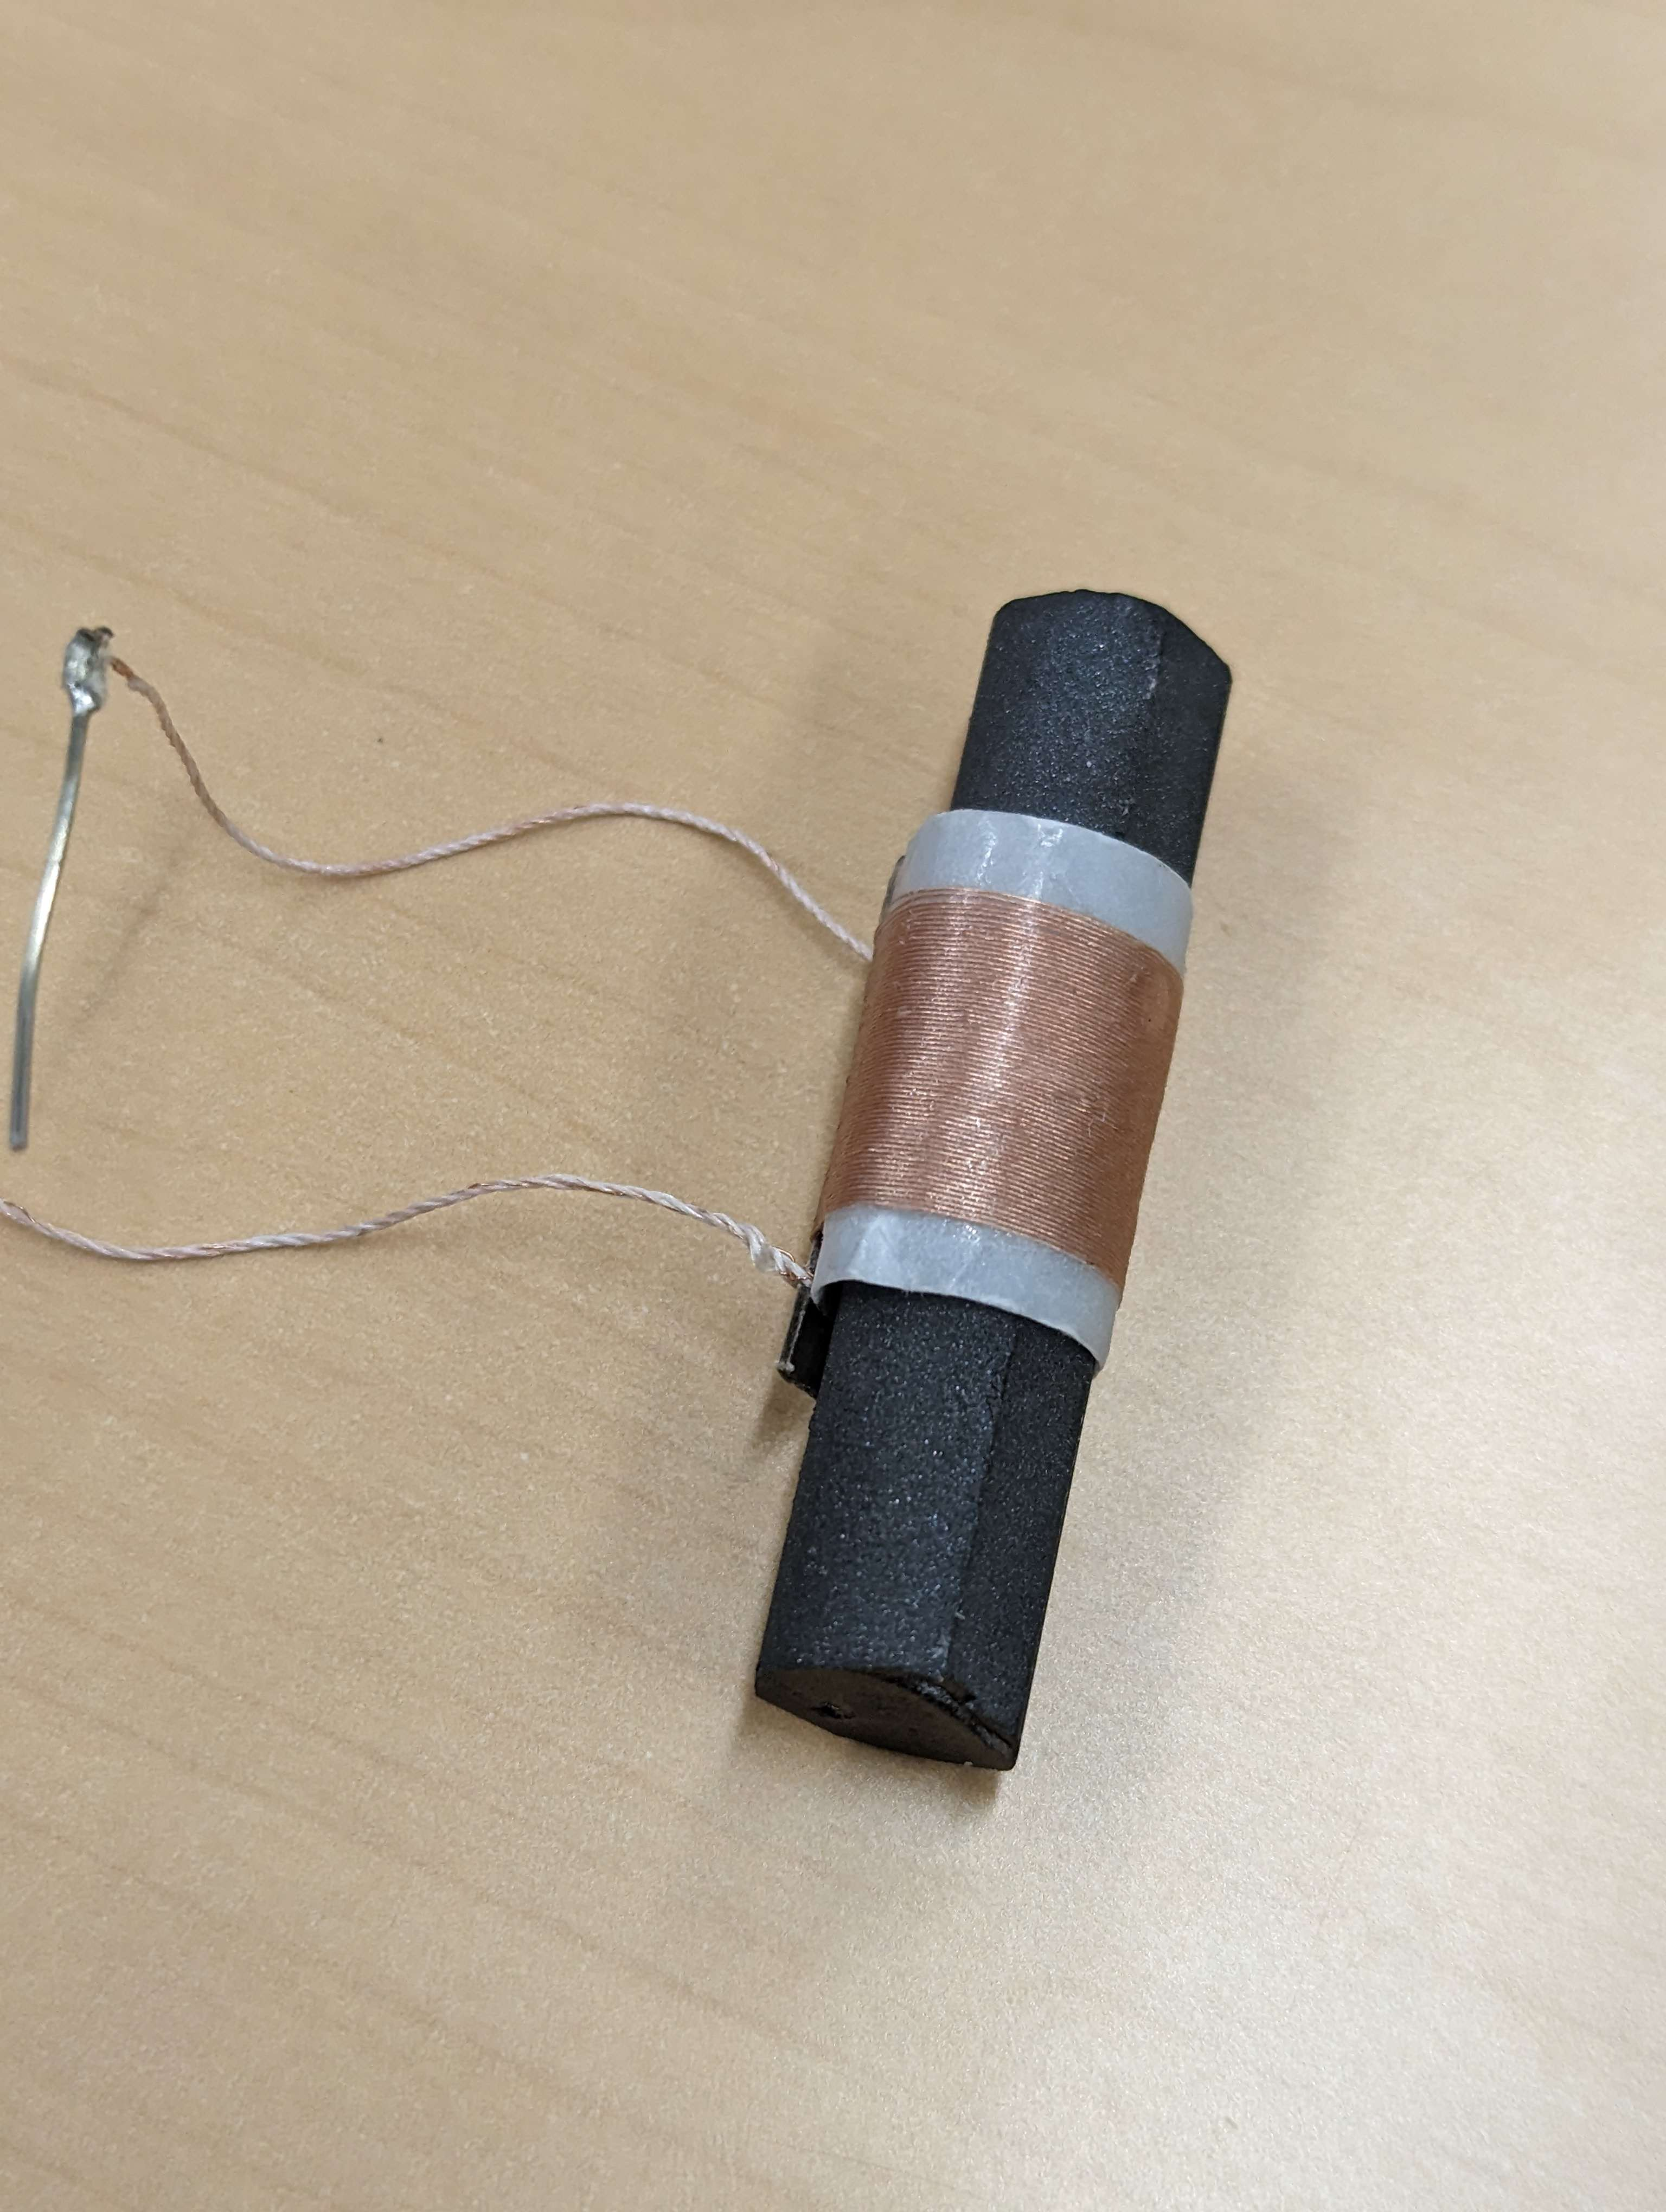
\includegraphics[width=7cm]{fig/3.jpg}
		\caption{3号機アンテナの写真}
		\label{fig:3}
	\end{minipage}
\end{figure}

それぞれのインダクタンスの測定は、\wfig{inda}のような回路を用いて行った。
周波数を変更させて、共振回路間の電圧を測定し、分圧則より共振周波数の場合はインピーダンスがほぼ無限になるため、5Vの電圧が測定できる。
5Vになった周波数から、\weq{resonance}と共振回路内のセラミックコンデンサ150 pFの値を用いて、インダクタンスを計算した。

\begin{figure}[H]
	\centering
	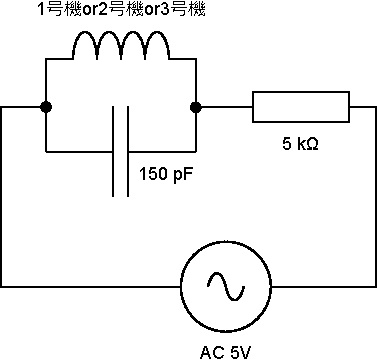
\includegraphics[width=10cm]{fig/inda.pdf}
	\caption{インダクタンス測定回路}
	\label{fig:inda}
\end{figure}

\wfig{inda2}に、\wfig{inda}の測定結果を示す。
1号機(Unit 1)と2号機(Unit2)は5.00 Vが計測できたが、3号機(Unit3)は4.31 Vまでしか計測できなかった。
また、\wfig{inda2}には載せていないが、3号機のフェライトを抜いたら共振しなくなり、0 Vが観測された。

\begin{figure}[H]
	\centering
	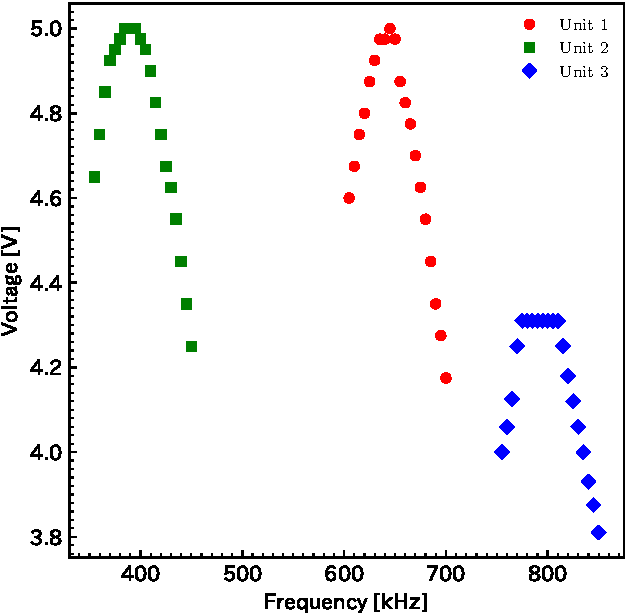
\includegraphics[width=10cm]{fig/1_kyo.pdf}
	\caption{インダクタンス測定回路の結果}
	\label{fig:inda2}
\end{figure}

\wfig{inda2}の結果から、\wtab{ant2}のように、インダクタンスと受信できる周波数を計算した。
受信できる周波数は、4 pF \(\sim\) 260 pFのバリアブルコンデンサを用いることを想定している。

\begin{table}[h]
	\centering
	\caption{インダクタンス測定回路}
	\label{tab:ant2}
	\begin{tabular}{ccccc} \hline
		名称  & 最大電圧[V] & 共振周波数[kHz] & インダクタンス[\(\upmu\)H] & 受信できる周波数[kHz]           \\ \hline
		1号機 & 5.00    & 約645       & 405.91              & 489.91 \(\sim\) 3949.80 \\
		2号機 & 5.00    & 約390       & 1110.24             & 296.23 \(\sim\) 2388.26 \\
		3号機 & 4.31    & 約790       & 270.58              & 600.69 \(\sim\) 4842.93 \\ \hline
	\end{tabular}
\end{table}

実際に、それぞれのアンテナで音を聞くと、

\begin{itemize}
	\item 1号機は1242 kHzのニッポン放送ははっきり聞こえるが
\end{itemize}

\subsubsection{受信強度}
アンテナをラジオ回路に接続したときの,クリスタルイヤホンからの音量によって,受信強度を評価した。一号機ではかすかに聞こえる(内容の把握はまれに可能である)ほどであり,二号機,三号機ではほとんど聞こえなかった。
\subsubsection{指向性}
上記回路で,アンテナを置く位置,向きを変更したときの,クリスタルイヤホンからの音量によって,指向性を評価した。一号機に関する結果を述べる。CAD室の窓際に置き,送信局へ向けた時最大の音量となった。それ以外の条件ではほとんど聞こえなかった。二号機,三号機に関しては評価を実施していない。

\subsection{ラジオ回路}
ラジオ回路の評価は難航した。回路にかかる電圧は微小信号であり,オシロスコープや電圧計での測定ができない。そのため,アンプで増幅してから評価するか,やはり出力された音声による評価を行う他なかった。

ラジオ回路に対し我々が行った評価は,アンテナ→ラジオ回路→スピーカーという風に出力したときの音声に含まれるノイズを

\subsection{アンプ}

\wfig{gain}に、今回用いた増幅回路のゲイン線図を示す。
\wfig{gain}のTheoretical valueが理想値(5.7倍、15.1175[dB])である。
Lowest rangeが人間が聞こえる周波数の最低値(20[Hz])である。
Highest rangeが人間が聞こえる周波数の最高値(20000[Hz])である。
測定値は、オシロスコープから取り出した波形のCSVファイルから最大値を取り出したものなので、
ノイズなどでゲインが少し理想値よりも高くなっている。
\(10^6\)[Hz]付近で、リップルが発生しており、その後に急激に減少している。
しかし、この領域は人間が聞こえる周波数の範囲外のため、問題ないと考えられる。
逆に、人間が聞こえる周波数の範囲内は、理想値に近い値を取っているため良いと考えられる。

\begin{figure}[H]
	\centering
	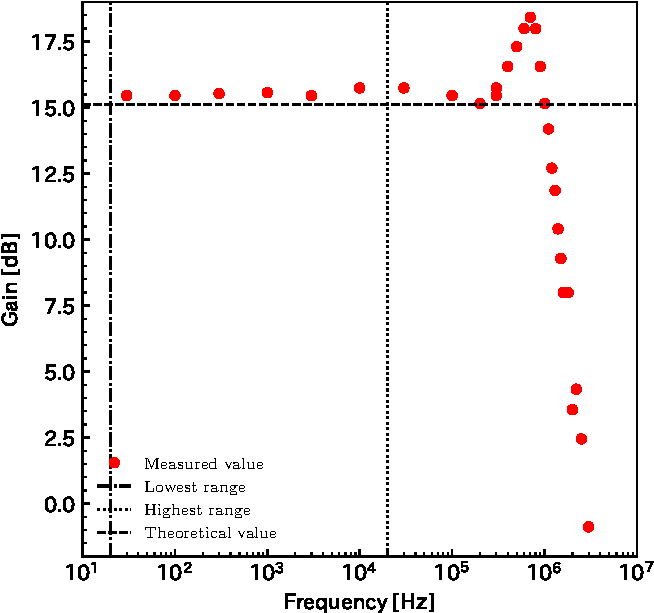
\includegraphics[width=10cm]{fig/gain.pdf}
	\caption{アンプのゲイン線図}
	\label{fig:gain}
\end{figure}

\end{document}
